% LOAD PACKAGES
\usepackage{amsmath} % allows for align env and other things
\usepackage{graphicx} % allows for graphics
\usepackage{textcomp} % allows for single apostrophe
%\usepackage{enumitem} % allows for alpha lettering in enumerated lists
\usepackage{amsfonts} % for real numbers symbol and other sets
\usepackage[mathscr]{euscript} % Euler script font
\usepackage{wrapfig} % to allow text wrapping
\usepackage{mathtools}
\usepackage{multirow}
\usepackage{pgfplots} % for surfaces (chapter 7), 2D graphics, etc
\usepackage{tikz-3dplot} 
\pgfplotsset{compat=1.9}
\usepackage{colortbl}
\usepackage{array}
% ~ ~ ~ ~ ~ ~ ~ ~ ~ ~ ~ ~ ~ ~ ~ ~ ~ ~ ~ ~ ~ ~ ~ ~ ~ ~ ~ 
% FONT
\usefonttheme[onlymath]{serif} %makes math characters serif, but also increases size of non-math characters
% ~ ~ ~ ~ ~ ~ ~ ~ ~ ~ ~ ~ ~ ~ ~ ~ ~ ~ ~ ~ ~ ~ ~ ~ ~ ~ ~ 
% CUSTOMIZED EMPHASIS
\definecolor{Black}{rgb}{0.0,0.0,0.0} % 
\definecolor{Teal}{rgb}{0.1,0.2,0.4}% 
\definecolor{Grey}{rgb}{0.4,0.4,0.4} % 
\newcommand{\Emph}[1]{{\color{Teal}\textbf{#1}}} % not needed
\DeclareTextFontCommand{\emph}{\bfseries\em}
% ~ ~ ~ ~ ~ ~ ~ ~ ~ ~ ~ ~ ~ ~ ~ ~ ~ ~ ~ ~ ~ ~ ~ ~ ~ ~ ~ 
% HEADER STYLE 
% THIS IS THE COLOR OF HEADER BAR ON TOP OF LECTURE SLIDES
\definecolor{HeaderBlue}{rgb}{0.051,0.051,0.051} % 
% Header Font Style
\setbeamerfont{frametitle}{size=\large\bfseries\color{Teal}}
% HEADER SPACING
\setbeamertemplate{headline}{\vskip3pt} % SPACE ABOVE HEADER
\addtobeamertemplate{frametitle}{}{\vspace*{0.3cm}} % SPACE AFTER HEADER
% ~ ~ ~ ~ ~ ~ ~ ~ ~ ~ ~ ~ ~ ~ ~ ~ ~ ~ ~ ~ ~ ~ ~ ~ ~ ~ ~ 
% COLORS FOR DIAGRAMS
\definecolor{DarkBlue}{rgb}{0.0,0.0,0.6} % 
\definecolor{DarkGreen}{rgb}{0.0,0.3,0.0} % 
\definecolor{DarkRed}{rgb}{0.6,0.0,0.0} % 
\definecolor{LightBlue}{rgb}{0.0,0.5,1.0} % 
\definecolor{Orange}{rgb}{1.0,0.5,0.0} % 
\definecolor{Gold}{rgb}{0.8,0.6,0.1} % 
\definecolor{LightGreen}{rgb}{0.3,0.9,0.3} % 
% ~ ~ ~ ~ ~ ~ ~ ~ ~ ~ ~ ~ ~ ~ ~ ~ ~ ~ ~ ~ ~ ~ ~ ~ ~ ~ ~ 
% FORMATTING OF BULLET AND ENUMERATED LISTS
\setbeamertemplate{itemize item}{$\bullet$}
\setbeamertemplate{itemize subitem}{$\bullet$}
\setbeamercolor{itemize item}{fg=Teal}
\setbeamercolor{itemize subitem}{fg=Teal}
% \setbeamercolor{itemize subitem}{fg=gray}
\setbeamercolor{enumerate item}{fg=Teal}
\setbeamercolor{enumerate subitem}{fg=gray}
% ~ ~ ~ ~ ~ ~ ~ ~ ~ ~ ~ ~ ~ ~ ~ ~ ~ ~ ~ ~ ~ ~ ~ ~ ~ ~ ~ 
% Topic and Learning Objective Statement
\newcommand{\LO}{\Emph{\color{Teal}Learning Objectives}}
\newcommand{\TopicStatement}{We will explore the following concepts in this video.}
\newcommand{\LearningObjectiveStatement}{After watching this video you should be able to:}
\newcommand{\LearningObjectiveStatementModule}{After completing the learning activities in this module students should be able to do the following.}
\newcommand{\LearningObjectiveStatementCourse}{After completing the learning activities in this course students should be able to do the following.}

\newcommand{\SummaryLine}{We explored the following concepts in this video.}
% ~ ~ ~ ~ ~ ~ ~ ~ ~ ~ ~ ~ ~ ~ ~ ~ ~ ~ ~ ~ ~ ~ ~ ~ ~ ~ ~ 
% COLORS IN LECTURE TITLE SLIDES 
%(the slide that appears at start of each lecture)
\setbeamercolor{frametitle}{fg=Black}
\setbeamercolor{slidetitle}{fg=Black}
\setbeamercolor*{title}{fg=black!80} % color of title slide title
% ~ ~ ~ ~ ~ ~ ~ ~ ~ ~ ~ ~ ~ ~ ~ ~ ~ ~ ~ ~ ~ ~ ~ ~ ~ ~ ~ 
% TITLE SLIDES 
\newcommand{\Course}{\textbf{Linear Algebra}}
\newcommand{\Instructor}{{\large {\color{Gold}{Greg Mayer, Ph.D.}}}\\[2pt] Academic Professional\\{\small {\color{gray} School of Mathematics}}}
\setbeamercolor{title}{fg=black}
\setbeamercolor{subtitle}{fg=Teal}
\setbeamertemplate{title page}[default][left,colsep=-12bp,rounded=true]
% ~ ~ ~ ~ ~ ~ ~ ~ ~ ~ ~ ~ ~ ~ ~ ~ ~ ~ ~ ~ ~ ~ ~ ~ ~ ~ ~ 
% COLORED CIRCLES FOR DIAGRAMS
\newcommand{\RedCircle}[2][black,fill=DarkRed]{\tikz[baseline=-0.5ex]\draw[#1,radius=#2] (0,0) circle ;}%
\newcommand{\BlueCircle}[2][black,fill=LightBlue]{\tikz[baseline=-0.5ex]\draw[#1,radius=#2] (0,0) circle ;}%
\newcommand{\GreenCircle}[2][black,fill=LightGreen]{\tikz[baseline=-0.5ex]\draw[#1,radius=#2] (0,0) circle ;}%
\newcommand{\OrangeCircle}[2][black,fill=Orange]{\tikz[baseline=-0.5ex]\draw[#1,radius=#2] (0,0) circle ;}%
% ~ ~ ~ ~ ~ ~ ~ ~ ~ ~ ~ ~ ~ ~ ~ ~ ~ ~ ~ ~ ~ ~ ~ ~ ~ ~ ~ 
% COLOURED BOXES FOR DEFINITIONS AND THEOREMS
\usepackage{tikz}
\usetikzlibrary{shapes,snakes}   
\usetikzlibrary{arrows,automata}
% ~ ~ ~ ~ ~ ~ ~ ~ ~ ~ ~ ~ ~ ~ ~ ~ ~ ~ ~ ~ ~ ~ ~ ~ ~ ~ ~ 
% WATERMARKS
\usepackage{lipsum}
\usepackage{tikz}
\setbeamertemplate{background}{%
\begin{tikzpicture}[overlay,remember picture]
\node[anchor=north west,scale=1.5] at ([shift={(-0.2in,0.2in)}]current page.north west) {
\includegraphics[width=0.4\textwidth]{images/GTHexes.png} };
\node[anchor=north west,scale=0.25] at ([shift={(5.5in,-0.1in)}]current page.north west) {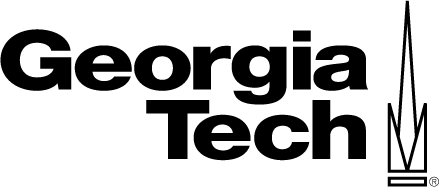
\includegraphics[width=0.4\textwidth]{images/GT-Logo.png} };
\end{tikzpicture}%
}
% ~ ~ ~ ~ ~ ~ ~ ~ ~ ~ ~ ~ ~ ~ ~ ~ ~ ~ ~ ~ ~ ~ ~ ~ ~ ~ ~ 
% REMOVE NAV BAR
\beamertemplatenavigationsymbolsempty
% ~ ~ ~ ~ ~ ~ ~ ~ ~ ~ ~ ~ ~ ~ ~ ~ ~ ~ ~ ~ ~ ~ ~ ~ ~ ~ ~ 
% CUSTOM TITLE SLIDE FOR GTPE
\setbeamertemplate{title page}{%
  \vbox{}
    \begin{flushleft}
    \begin{beamercolorbox}[sep=8pt]{title}
      \usebeamerfont{title}{\textbf{\insertinstitute}}\par%
      \ifx\insertsubtitle\@empty%
      \else%
        \vskip0.25em%
        {\usebeamerfont{subtitle}\usebeamercolor[fg]{subtitle}\insertsubtitle\par}%
      \fi%     
    \end{beamercolorbox}%
    \vskip1em\par
    \vfill%<- added
    \begin{beamercolorbox}[sep=8pt]{author}
      \usebeamerfont{author}\insertauthor
    \end{beamercolorbox}
    \vfill%<- added
    \begin{beamercolorbox}[sep=8pt]{institute}
      \usebeamerfont{institute}{{\color{Teal}\Large \inserttitle}}
    \end{beamercolorbox}
    \end{flushleft}
}
% ~ ~ ~ ~ ~ ~ ~ ~ ~ ~ ~ ~ ~ ~ ~ ~ ~ ~ ~ ~ ~ ~ ~ ~ ~ ~ ~ 
% ASPECT RATIO
\usepackage[orientation=landscape,size=custom,width=16,height=9,scale=0.5,debug]{beamerposter} 
% ~ ~ ~ ~ ~ ~ ~ ~ ~ ~ ~ ~ ~ ~ ~ ~ ~ ~ ~ ~ ~ ~ ~ ~ ~ ~ ~ 
% MATH THING: AUGMENTED MATRIX
% augmeted matrix environment, from Hefferon
\newenvironment{amatrix}[1]{%
  \left(\begin{array}{@{}*{#1}{c}|c@{}}
}{%
  \end{array}\right)
}
% ~ ~ ~ ~ ~ ~ ~ ~ ~ ~ ~ ~ ~ ~ ~ ~ ~ ~ ~ ~ ~ ~ ~ ~ ~ ~ ~ 
% OTHER MATH THINGS
\newcommand{\R}{{\mathbb R}} % The real numbers
\usepackage{spalign} % Joe Rabinoff's matrix package
% SUBSPACES AND ORTHOGONALITY
\newcommand{\Perp}{^{\perp}}
\newcommand{\Row}{\text{Row}}
\newcommand{\Col}{\text{Col}}
\newcommand{\Nul}{\text{Nul}}
\newcommand{\Null}{\text{Nul}}
\newcommand{\proj}{\text{proj}}
\newcommand{\Span}{\text{Span}}
\newcommand{\Rank}{\text{rank}}

\usetikzlibrary{decorations.pathreplacing,calligraphy, matrix, backgrounds, positioning, calc}
